\section{JPA Entity Manager}

In JPA, entity instances are POJOs that only become managed when an API method is invoked to start the process. 
The Entity Manager is the central authority for all persistence actions, handling the mapping and APIs for database interactions.
\begin{definition}[\textit{Persistence context}]
    The persistence context is a core concept in JPA, acting like a main memory database that holds objects in a managed state.
\end{definition}
A managed object is tracked, enabling automatic synchronization of its state modifications with the database. 
Database writes generally occur asynchronously, requiring the persistence context to connect to a transaction when they happen. 
A managed entity has dual lives: one as a Java object and one as a relational tuple, existing only within the persistence context. 
When the POJO exits the persistence context, the binding breaks, and it is no longer tracked or synchronized with the database.
Applications interact with the Entity Manager, not directly with the persistence context.

\subsection{Operations}
When an entity is first instantiated, it is in a transient state because the Entity Manager is not aware of its existence. 
Transient entities are not part of the persistence context associated with the Entity Manager.
\begin{example}
    A new POJO can be created as follows:
\begin{lstlisting}[style=Java]
Employee emp = new Employee(ID, "John Doe"); 
\end{lstlisting}
\end{example}
To transition transient entities to the managed state, the \texttt{persist()} method of the Entity Manager is used. 
Once an entity becomes managed, any changes made to it are automatically applied to the database. 
The managed entity and its corresponding tuple are associated until the entity exits the managed state.
You can call \texttt{persist()} on an already managed entity to trigger the cascade process.
\begin{example}
    A new POJO can be created and later made managed as follows:
\begin{lstlisting}[style=Java]
Employee emp = new Employee(ID, "John Doe"); 
em.persist(emp);
\end{lstlisting}
\end{example}
Entities can be retrieved using the \texttt{find()} method, which takes the class of the sought entity and the primary key value identifying the desired entity instance. 
If the entity instance is found, the returned object becomes managed; otherwise, the \texttt{find()} method returns null.
\begin{example}
    Finding an entity: 
\begin{lstlisting}[style=Java]
Employee emp = em.find(Employee.class, ID);
\end{lstlisting}
\end{example}
To remove an entity, the \texttt{remove()} method is used.
This action breaks the association between the entity and the persistence context. 
Upon the transaction associated with the Entity Manager's persistence context committing, or when the \texttt{flush()} method of the Entity Manager is called, the tuple linked with the entity is scheduled for deletion from the database. 
Although the entity still exists, its changes are no longer tracked for synchronization with the database.
\begin{example}
    Removing an entity:
\begin{lstlisting}[style=Java]
em.remove(emp);
\end{lstlisting}
\end{example}
\begin{figure}[H]
    \centering
    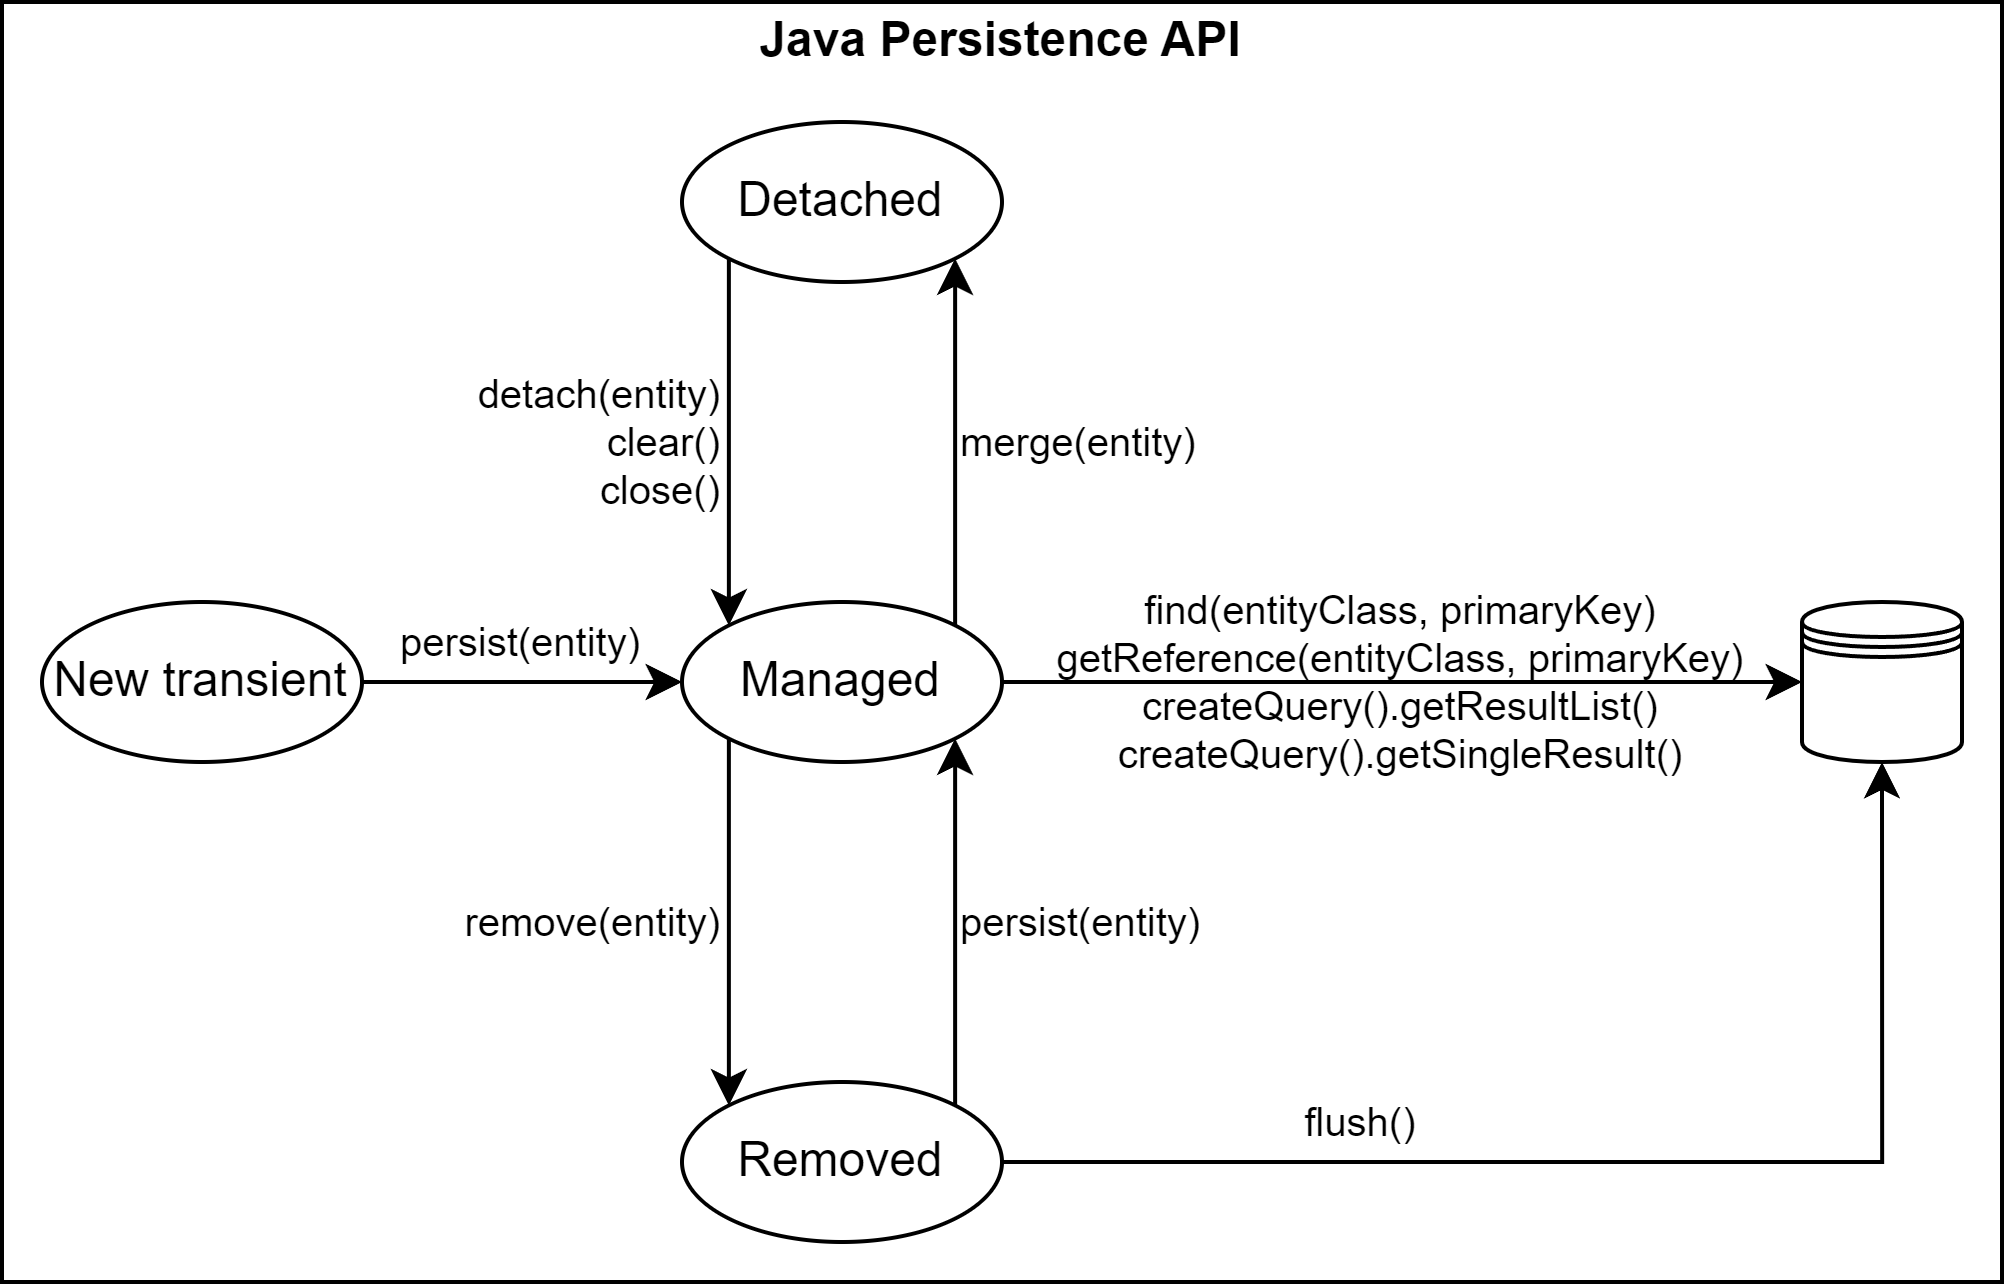
\includegraphics[width=0.75\linewidth]{images/jpaem.png}
    \caption{Possible states for the entities}
\end{figure}
Referring to the preceding diagram, entities can exist in five primary states:
\begin{itemize}
    \item \textit{New}: the entity is unknown to the Entity Manager, lacks a persistent identity, and has no associated tuple.
    \item \textit{Managed}: the entity is associated with the persistence context, and changes to objects are automatically synchronized with the database.
    \item \textit{Detached}: the entity has an identity potentially associated with a database tuple, but changes are not automatically propagated to the database.
    \item \textit{Removed}: the entity is scheduled for removal from the database.
    \item \textit{Deleted}: the entity is erased from the database.
\end{itemize}

\subsection{Application architecture}
In JEE, clients leverage the services of the EJB container to establish a connection with the Entity Manager.
Specifically, the business layer interacts with the Entity Manager.
The advantage of using EJB is that the container provides support to make JPA entity method calls transactional through the automatic creation of transactions.
\begin{figure}[H]
    \centering
    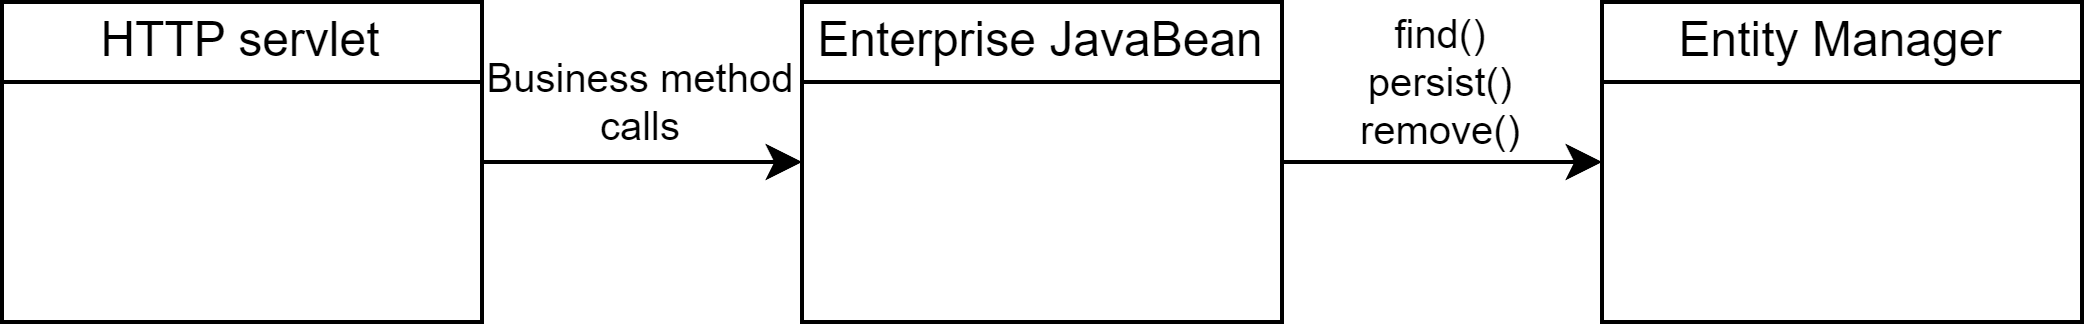
\includegraphics[width=0.75\linewidth]{images/jee1.png}
\end{figure}
Transactions in this context exist at three levels:
\begin{itemize}
    \item \textit{DBMS transactions}: managed by the DBMS and utilize SQL. 
        This level is used by the Entity Manager.
    \item \textit{Resource-local transactions}: managed by the application and use the JDBC connection interface, mapped to JDBC.
    \item \textit{Container transaction}: managed by the application or the container and use the JTA interface, also mapped to JDBC. 
        The Entity Manager operates at this level.
\end{itemize}
After defining a business object, the container injects the Entity Manager into it. 
The container transparently manages instances of the Entity Manager for the application. 
It provides the transaction required to save modifications made to the entities in the persistence context associated with the Entity Manager into the database.
\begin{example}
    Definition of a business object EJB: 
\begin{lstlisting}[style=Java]
@Stateless 
public class myEJBService {
    @PersistenceContext(unitName = "MyPersistenceUnit")
    private EntityManager em; 
}
\end{lstlisting}
\end{example}
When a client calls a method of a business object that utilizes a container-managed entity manager for persistence, the container offers a transaction for saving modifications to the database. 
If the same transaction is called multiple times, it is reused. 
This behavior is the most common and default, but the business object methods can be annotated to specify a different transactional behavior using \texttt{@TransactionAttribute(TransactionAttributeType.type)}, where \texttt{type} can be: 
\begin{itemize}
    \item \texttt{Mandatory}: expects a transaction to have already been started and be active when the method is called. 
        If no transaction is active, an exception is thrown.
    \item \texttt{Required}: the default behavior; starts a new transaction if none is active.
        If one is active, it is used.
    \item \texttt{Requires\_new}: the method always needs to be in its own transaction. 
        Any active transaction is suspended.
    \item \texttt{Supports}: the method does not access transactional resources but tolerates running inside one if it exists.
    \item \texttt{Not\_supported}: the method will cause the container to suspend the current transaction if one is active when the method is called.
    \item \texttt{Never}: the method will cause the container to throw an exception if a transaction is active when the method is called.
\end{itemize}